% Left: the 15-puzzle in Loyd's position (14 and 15 swapped), on a checkerboard whose bottom-right cell is white.
% Right: the 7 conjugacy classes of S5 by cycle type, with their sizes; even classes dark, odd classes light. Generated by a short script.
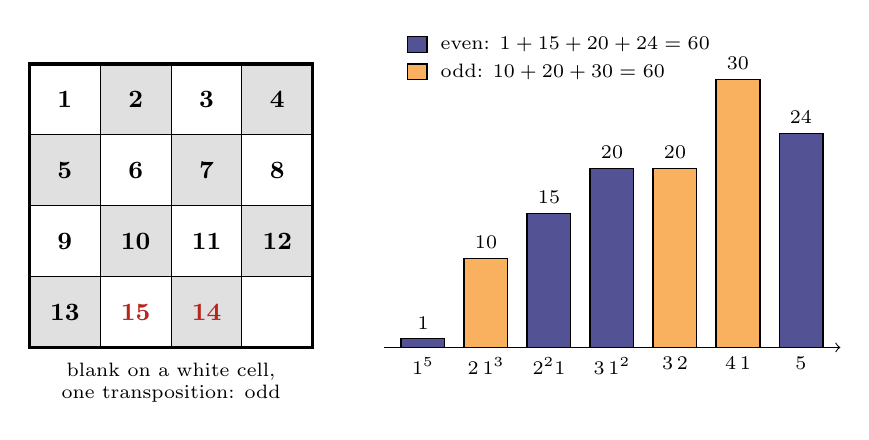
\begin{tikzpicture}
\filldraw[draw=black,fill=white] (0.00,2.70) rectangle (0.90,3.60);
\node[font=\small\bfseries,text=black] at (0.45,3.15) {1};
\filldraw[draw=black,fill=black!12] (0.90,2.70) rectangle (1.80,3.60);
\node[font=\small\bfseries,text=black] at (1.35,3.15) {2};
\filldraw[draw=black,fill=white] (1.80,2.70) rectangle (2.70,3.60);
\node[font=\small\bfseries,text=black] at (2.25,3.15) {3};
\filldraw[draw=black,fill=black!12] (2.70,2.70) rectangle (3.60,3.60);
\node[font=\small\bfseries,text=black] at (3.15,3.15) {4};
\filldraw[draw=black,fill=black!12] (0.00,1.80) rectangle (0.90,2.70);
\node[font=\small\bfseries,text=black] at (0.45,2.25) {5};
\filldraw[draw=black,fill=white] (0.90,1.80) rectangle (1.80,2.70);
\node[font=\small\bfseries,text=black] at (1.35,2.25) {6};
\filldraw[draw=black,fill=black!12] (1.80,1.80) rectangle (2.70,2.70);
\node[font=\small\bfseries,text=black] at (2.25,2.25) {7};
\filldraw[draw=black,fill=white] (2.70,1.80) rectangle (3.60,2.70);
\node[font=\small\bfseries,text=black] at (3.15,2.25) {8};
\filldraw[draw=black,fill=white] (0.00,0.90) rectangle (0.90,1.80);
\node[font=\small\bfseries,text=black] at (0.45,1.35) {9};
\filldraw[draw=black,fill=black!12] (0.90,0.90) rectangle (1.80,1.80);
\node[font=\small\bfseries,text=black] at (1.35,1.35) {10};
\filldraw[draw=black,fill=white] (1.80,0.90) rectangle (2.70,1.80);
\node[font=\small\bfseries,text=black] at (2.25,1.35) {11};
\filldraw[draw=black,fill=black!12] (2.70,0.90) rectangle (3.60,1.80);
\node[font=\small\bfseries,text=black] at (3.15,1.35) {12};
\filldraw[draw=black,fill=black!12] (0.00,0.00) rectangle (0.90,0.90);
\node[font=\small\bfseries,text=black] at (0.45,0.45) {13};
\filldraw[draw=black,fill=white] (0.90,0.00) rectangle (1.80,0.90);
\node[font=\small\bfseries,text=BrickRed] at (1.35,0.45) {15};
\filldraw[draw=black,fill=black!12] (1.80,0.00) rectangle (2.70,0.90);
\node[font=\small\bfseries,text=BrickRed] at (2.25,0.45) {14};
\filldraw[draw=black,fill=white] (2.70,0.00) rectangle (3.60,0.90);
\draw[very thick] (0,0) rectangle (3.60,3.60);
\node[font=\scriptsize,align=center] at (1.80,-0.45) {blank on a white cell,\\ one transposition: odd};
\draw[->] (4.50,0) -- (10.30,0);
\filldraw[draw=black,fill=MidnightBlue!75] (4.72,0) rectangle (5.27,0.11);
\node[font=\scriptsize,above] at (5.00,0.11) {1};
\node[font=\scriptsize,below] at (5.00,0) {$1^5$};
\filldraw[draw=black,fill=BurntOrange!60] (5.52,0) rectangle (6.07,1.13);
\node[font=\scriptsize,above] at (5.80,1.13) {10};
\node[font=\scriptsize,below] at (5.80,0) {$2\,1^3$};
\filldraw[draw=black,fill=MidnightBlue!75] (6.32,0) rectangle (6.87,1.70);
\node[font=\scriptsize,above] at (6.60,1.70) {15};
\node[font=\scriptsize,below] at (6.60,0) {$2^2 1$};
\filldraw[draw=black,fill=MidnightBlue!75] (7.12,0) rectangle (7.67,2.27);
\node[font=\scriptsize,above] at (7.40,2.27) {20};
\node[font=\scriptsize,below] at (7.40,0) {$3\,1^2$};
\filldraw[draw=black,fill=BurntOrange!60] (7.92,0) rectangle (8.47,2.27);
\node[font=\scriptsize,above] at (8.20,2.27) {20};
\node[font=\scriptsize,below] at (8.20,0) {$3\,2$};
\filldraw[draw=black,fill=BurntOrange!60] (8.72,0) rectangle (9.28,3.40);
\node[font=\scriptsize,above] at (9.00,3.40) {30};
\node[font=\scriptsize,below] at (9.00,0) {$4\,1$};
\filldraw[draw=black,fill=MidnightBlue!75] (9.53,0) rectangle (10.08,2.72);
\node[font=\scriptsize,above] at (9.80,2.72) {24};
\node[font=\scriptsize,below] at (9.80,0) {$5$};
\filldraw[draw=black,fill=MidnightBlue!75] (4.80,3.75) rectangle (5.05,3.95);
\node[font=\scriptsize,right] at (5.10,3.85) {even: $1+15+20+24=60$};
\filldraw[draw=black,fill=BurntOrange!60] (4.80,3.40) rectangle (5.05,3.60);
\node[font=\scriptsize,right] at (5.10,3.5) {odd: $10+20+30=60$};
\end{tikzpicture}
